\pdfoutput=1

\documentclass{article}
\usepackage{iclr2018}
\usepackage{times}
\usepackage{float}
\usepackage{hyperref}
\usepackage{url}
\usepackage{graphicx}
\usepackage{amsmath}
\usepackage{amsfonts}
\usepackage{subcaption}
\usepackage{listings}
\usepackage{lipsum}
\usepackage{microtype}
\usepackage{booktabs}
\usepackage{multirow}
\usepackage{siunitx}
\usepackage{hyphenat}

\usepackage{pifont}% http://ctan.org/pkg/pifont
\newcommand{\cmark}{\ding{51}}%
\newcommand{\xmark}{\ding{55}}%

\newcommand{\mixup}{\emph{mixup}}
\newcommand{\todo}[1]{{\color{red} TODO: {#1}}}
\DeclareMathOperator*{\E}{\mathbb{E}}
\newcommand*\samethanks[1][\value{footnote}]{\footnotemark[#1]}

\lstdefinestyle{mypython}{
  language=python,
  breaklines=true,
  basicstyle=\fontsize{8.5}{13}\selectfont\ttfamily,
  keywordstyle=\bfseries\color{green!40!black},
}

\iclrfinalcopy

\title{\mixup{}: Beyond Empirical Risk Minimization}

\author{%
Hongyi Zhang \\
MIT
\And
Moustapha Cisse, Yann N. Dauphin, David Lopez-Paz\thanks{Alphabetical order.} \\
FAIR
}

\begin{document}
    \maketitle
    \begin{abstract}
        Large deep neural networks are powerful, but exhibit undesirable
        behaviors such as memorization and sensitivity to adversarial examples.
        In this work, we propose \mixup{}, a simple learning principle to
        alleviate these issues. In essence, \mixup{} trains a neural network on
        convex combinations of pairs of examples and their labels.  By doing
        so, \mixup{} regularizes the neural network to favor simple linear
        behavior in-between training examples.  Our experiments on the
        ImageNet-2012, CIFAR-10, CIFAR-100, Google commands and UCI datasets
        show that \mixup{} improves the generalization of state-of-the-art
        neural network architectures.  We also find that \mixup{} reduces the
        memorization of corrupt labels, increases the robustness to adversarial
        examples, and stabilizes the training of generative adversarial
        networks.
    \end{abstract}
    \section{Introduction}
Despite the well-recognized importance of training data in advancing the capabilities of large language models (LLMs)~\cite{brown2020language,kaplan2020scaling,Razeghi2022ImpactOP}, there is no agreed-upon mechanisms for crediting or compensating data providers. As LLMs are increasingly integrated into our society and economy, the absence of such mechanisms has aggravated a tension between data and model providers, exemplified by recent legal challenges involving major tech companies~\cite{jlversusalphabet,metz2022lawsuit}. In this atmosphere, data valuation, which quantifies the contribution of each training data to the model output, has been discussed as a potential technical solution for tackling these societal issues~\cite{fernandez2023data,ghorbani2019data,huang2023citation,jia2019towards,worledge2023unifying,zhao2023addressing}. 

At a high level, most data valuation algorithms interpret the model output as a coalition of its training data, and evaluate the contribution of each example based on its influence on the model output when included or excluded from the training dataset~\cite{ghorbani2019data,ilyas2022datamodels,koh2017understanding,kwon2021beta}. If an inclusion of a specific training example consistently improves model performance, high value can be assigned to this example for its contribution. However, applying existing data valuation methods to recent LLMs and their vast training datasets has faced significant scalability challenges to date. For instance, sampling-based methods, such as the Shapley value~\cite{ghorbani2019data,kwon2021beta} or Datamodels~\cite{ilyas2022datamodels}, require retraining the model multiple times with varied combinations of data subsets to directly model the effect of in/excluding each data. Unfortunately, such repeated retraining is hardly affordable even for small models, let alone LLMs. To overcome this issue, gradient-based methods, including influence functions~\cite{koh2017understanding,park2023trak}, approximate the effect of data in/exclusion on the model output using gradient information without costly retraining. Even so, scaling gradient-based methods to LLMs is hindered by prohibitive compute and memory costs originating in the high-dimensional nature of the gradient.

Consequently, the main objective of this work is to bridge the gap in scaling existing data valuation methods to recent LLMs and their vast training datasets. Toward this goal, we focus on influence functions \cite{koh2017understanding,park2023trak}, a representative gradient-based data valuation method, and significantly improve its scalability with an efficient gradient projection algorithm. We visualize the proposed data valuation system in Figure~\ref{fig:diagram}, and detail our technical contributions below:

\begin{figure}
    \centering
    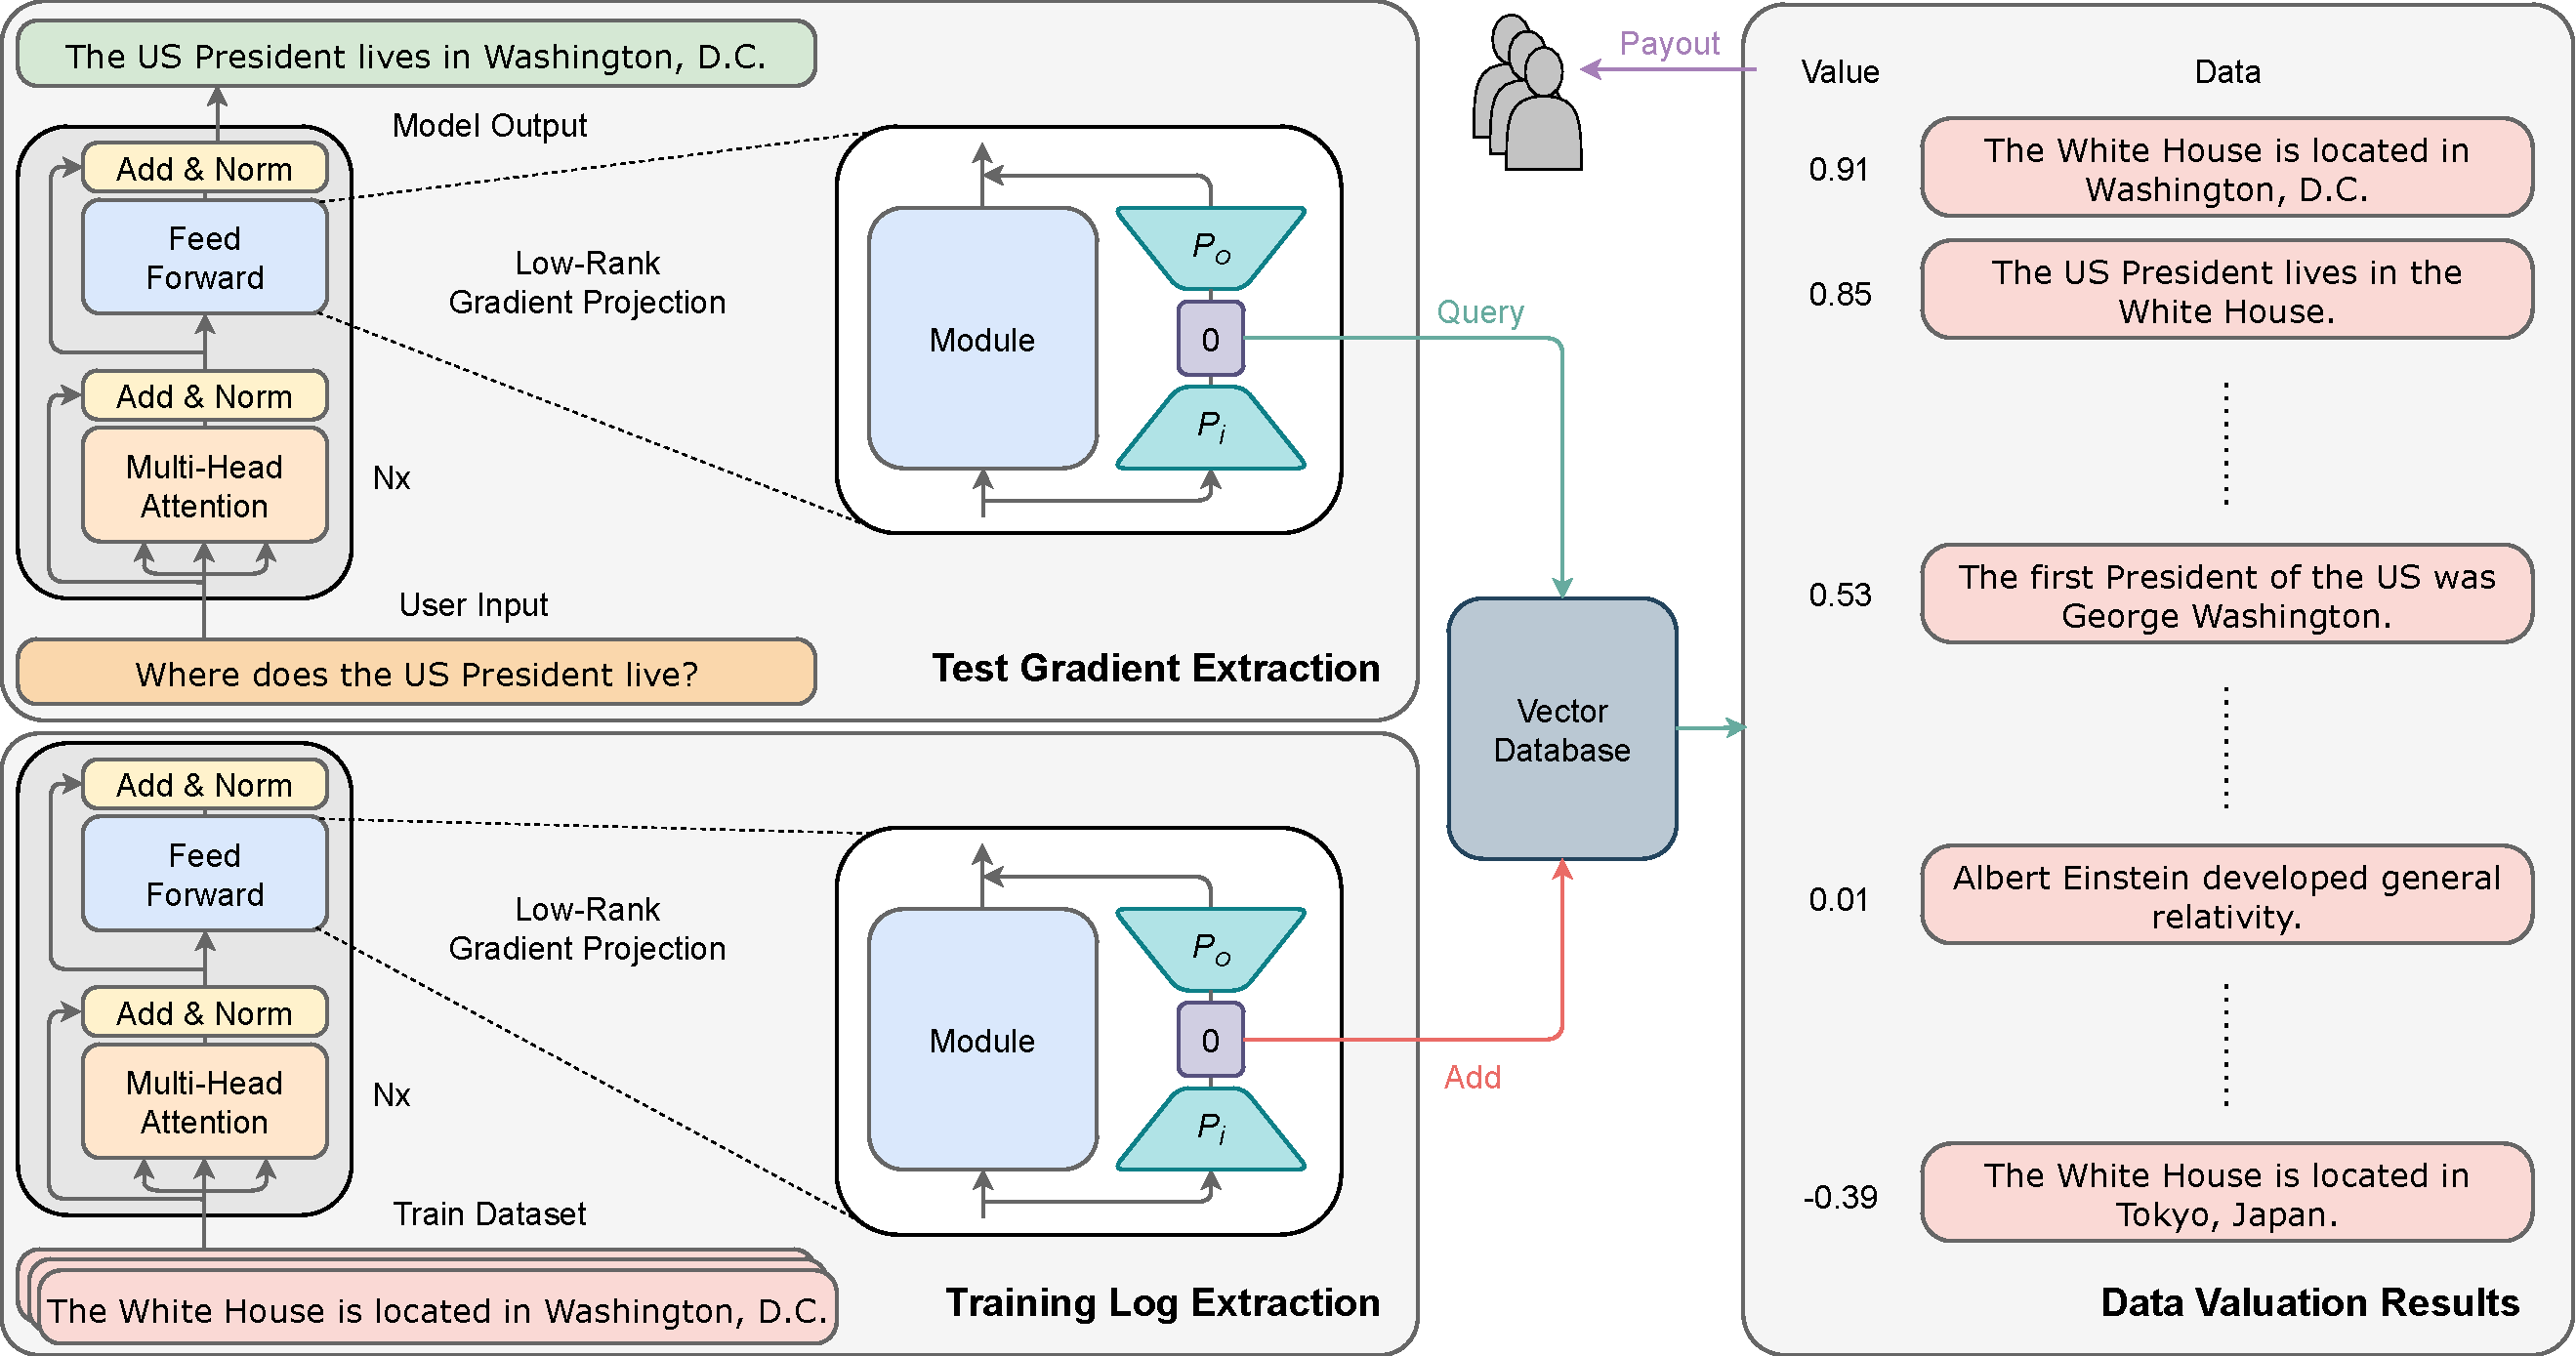
\includegraphics[width=0.94\textwidth]{figures/diagram_v7.pdf}
    \vskip -4pt
    \caption{Data valuation system architecture. \textbf{(Left Bottom)} We first extract the Hessian and gradients for all training data using efficient gradient projection \method\ and store them in a database. \textbf{(Left Top)} At test time, we similarly extract gradients and query the database. \textbf{(Right)} The database returns similarity scores with respect to training examples that can be used for data valuation/attribution.}
    \label{fig:diagram}
\end{figure}

\begin{itemize}[leftmargin=*,topsep=-2pt]
    \item Employing gradient structures in backpropagation, we develop a novel \textbf{lo}w-rank \textbf{gra}dient projection algorithm \method\ that improves space \& time complexity of gradient projection, a major scalability bottleneck in prior work~\cite{park2023trak,schioppa2022scaling}, from $O(nk)$ to $O(\sqrt{nk})$ where $n$ and $k$ are model and projection dimensions. Furthermore, \method\ directly computes projected gradients without materializing full gradients, enabling low GPU memory and high GPU utilization for improved efficiency. Lastly, we show that \method\ can be easily implemented with small add-on layers, similarly to LoRA~\cite{hu2021lora}.
    \item By interpreting a damping term in influence functions as a spectral gradient sparsification mechanism, we (1) offer a theoretical motivation of gradient projection approaches to influence functions and (2) derive a specialized PCA initialization scheme for \method.
    \item We introduce software named \software\ that (1) makes it \textit{simple} to convert existing training code into data valuation code, (2) is \textit{compatible} with various scalability tools and features in the LLM ecosystem, and (3) is \textit{extensible} to implement other data valuation or interpretability algorithms.
    \item In our data valuation experiments, \method\ demonstrates competitive accuracy against more costly baselines, while showing up to 6,500$\times$ increase in throughput and 5$\times$ reduction in GPU memory, when applied to Llama3-8B-Instruct~\cite{llama3modelcard} and the 1B-token dataset, compared to EKFAC influence \cite{grosse2023studying}, the state-of-the-art and only runnable baseline at this scale. We also observe that most valuable data identified by \method\ generally share qualitative similarities with the queried LLM output.
\end{itemize}
    \begin{figure}[t]
    \centering
    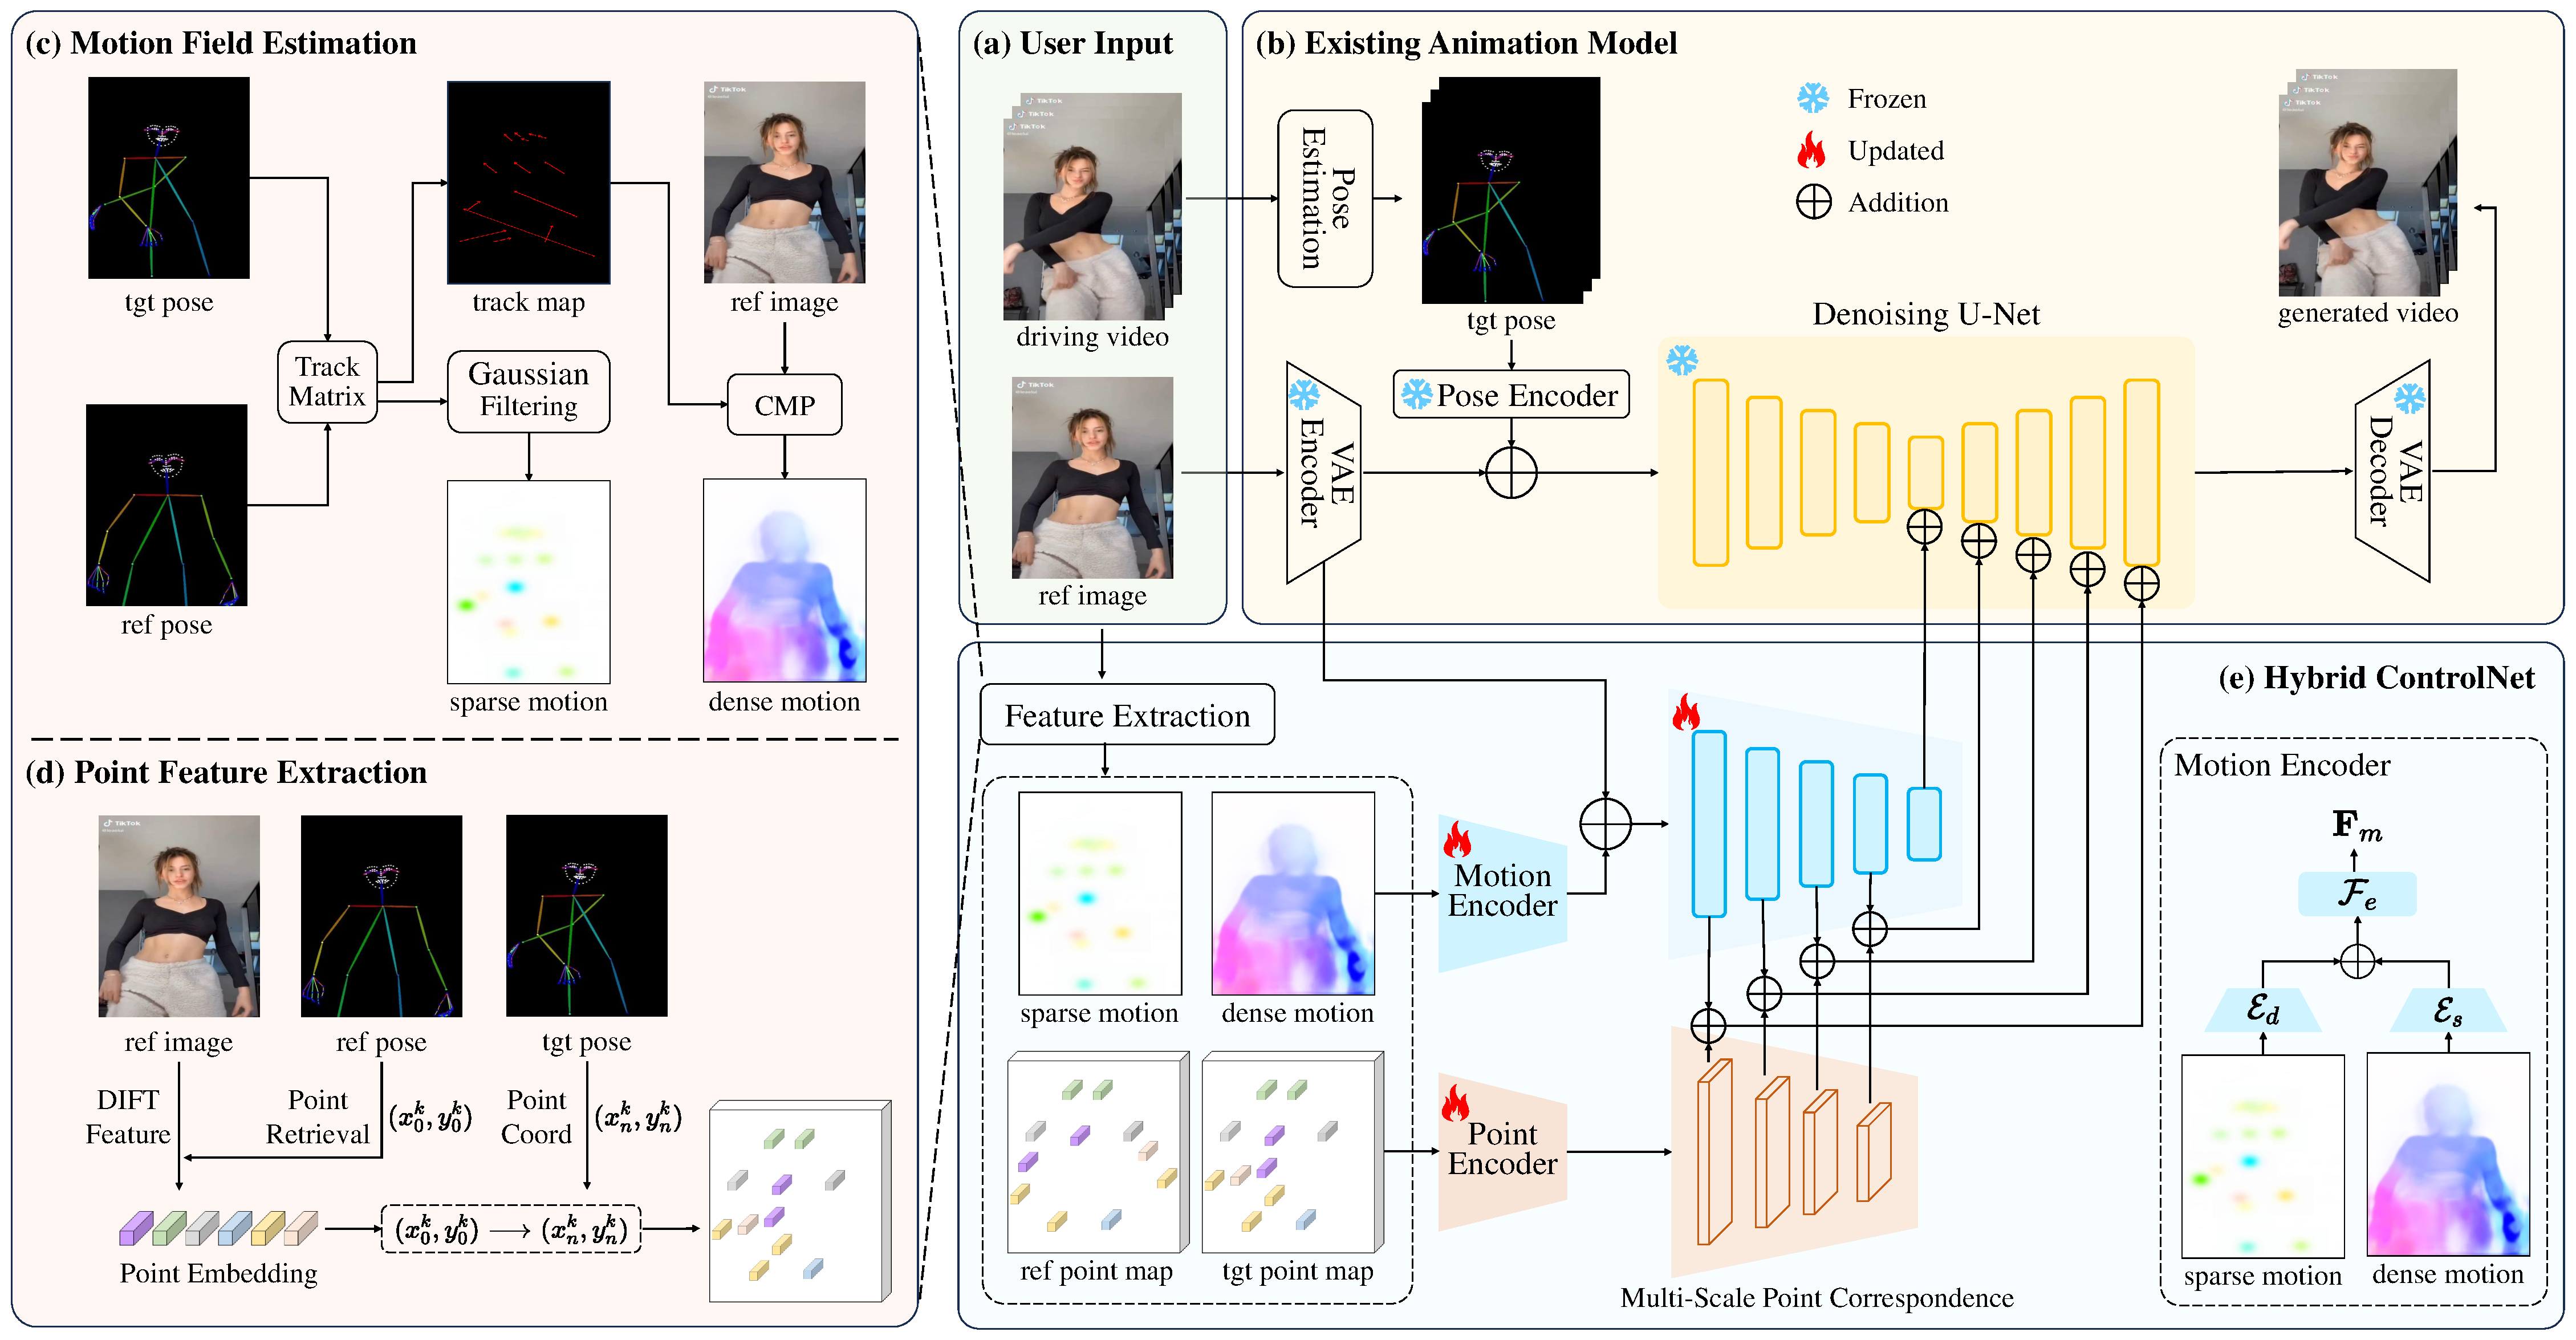
\includegraphics[width=1.0\columnwidth]{./image/pipeline.pdf}
    \vspace{-15pt}
    \caption{The overview of proposed DisPose.}
    \label{fig:pipeline}
\end{figure}
\section{DisPose}
Given a reference image $I_{\mathrm{ref}}\!\in\!\mathbb{R}^{3 \times H \times W}$ and a driving video $V\!\in\!\mathbb{R}^{N\times 3 \times H \times W}$. The core of our method is to disentangle efficient control guidance from only skeleton poses and reference images as shown in Figure~\ref{fig:pipeline}, which can be applied to existing human animation methods without additional dense inputs. We first introduce sparse and dense motion field guides in Sec.~\ref{sec: motion}. Then, we introduce reference-based keypoint correspondence in Sec.~\ref{sec: keypoint}. Finally, we introduce the pipeline of hybrid ControlNet in Sec~\ref{sec: controlnet}.
\subsection{Motion Field Guidance}
\label{sec: motion}

\textbf{Sparse Motion Field.}
We first estimate the skeleton pose by DWpose~\citep{yang2023dwpose} to obtain each frame's human key point coordinates. 
% Subsequently, the motion trajectory of all semantic points in the entire video is obtained and represented as
Subsequently, the key points of the reference image are used as starting points to track the motion displacement of all frames and represented as $P_{traj}\!=\!\{(x^k_n,y^k_n) \!\mid\! k=1\dots K, n=0\dots N\}$, where $P_{traj}$ denotes the trajectory map of the key point $k$ overall $N$ frames and $n = 0$ denotes the reference image. We calculate the track matrix $P_{s}$ as follows:
\begin{equation}
    \mathbf{P}_{s}=\{(x^k_n-x^k_{n-1}, y^k_n-y^k_{n-1}) \mid n=1\dots N\}\},
\end{equation}
% where $P_{t}$ denotes the trajectory map of the key point point $k$ over all $N$ frames, and the reference frame when $n = 0$.
where $K$ denotes the number of keypoints, $N$ denotes the number of frames, $\mathbf{P}_{s}$ denotes the trajectory map of keypoint k over all N frames, and $n = 0$ denotes the reference image.
To avoid training instability caused by overly sparse trajectory matrice, we then apply Gaussian filtering to enhance $\mathbf{P}_{s}$ to obtain the sparse motion field $\mathbf{F}_s\!\in\!\mathbb{R}^{(N-1)\times 2 \times H \times W}$ inspired by~\citep{yin2023dragnuwa, wang2024motionctrl}.

\textbf{Dense Motion Field.}
Considering that sparse control provides limited guidance and dense control is hard to obtain during inference,
% For the dense motion field, 
we transform dense guidance into the motion propagation from the reference frame to the target pose, instead of the dense signal of the target pose. Specifically, in the inference, we reconstruct the trajectory map $\mathbf{P}_{s}$ as the reference-based sparse optical flow $\mathbf{P}_{d}$ from the reference frame to each target pose as:
\begin{equation}
    \mathbf{P}_{d}=\{(x^k_n-x^k_{0}, y^k_n-y^k_{0}) \mid n=1\dots N\}\},
\end{equation}
We then predicted the reference-based dense motion filed $\mathbf{F}_d\!=\! \text{CMP}(P_{traj}, \mathbf{P}_{d}, I_{ref})\!\in\!\mathbb{R}^{(N-1)\times 2 \times H \times W}$ by condition motion propagation (CMP)~\citep{zhan2019self} based on the sparse optical flow $\mathbf{P}_{d}$ and the reference image $I_{ref}$.
CMP~\citep{zhan2019self} is a self-supervised learning-from-motion model that acquires an image and a sparse motion field and estimates the corresponding dense motion field.
Notably, the dense motion field $\mathbf{F}_d$ of each frame starts with the reference image, which avoids geometric constraints during inference.

To ensure motion estimation accuracy during training, we first extract the forward optical flow from the driving video using existing optical flow estimation models~\citep{teed2020raft, xu2023unifying}. We then use a watershed-based approach~\citep{zhan2019self} to sample the sparse optical flow $\mathbf{P}_{d}$ from the forward optical flow. See Appendix.~\ref{sec: appendix1} for details.

\textbf{Motion Encoder.} To leverage motion field as guidance, we introduce a motion encoder specifically designed for the optional flow, which includes sparse motion encoder $\mathcal{E}_s$, dense motion encoder $\mathcal{E}_d$ and feature fusion layer $\mathcal{F}_e$. $\mathcal{E}_d$ and $\mathcal{E}_s$ have the same structure and are multi-scale convolutional encoders with each stage built by \texttt{Conv-SiLU-ZeroConv}~\citep{zhang2023adding} as the basic block. The feature fusion layer $\mathcal{F}_e$ is a 2D convolution for fusing sparse motion features $\mathcal{E}_s(\mathbf{F}_s)$ and dense motion features $\mathcal{E}_d(\mathbf{F}_d)$. Finally, we compute the motion field guidance $\mathbf{F}_m$:
\begin{equation}
    \mathbf{F}_m = \mathcal{F}_e(\mathcal{E}_s(\mathbf{F}_s)+\mathcal{E}_d(\mathbf{F}_d))
\end{equation}

\subsection{Keypoint Correspondence}
\label{sec: keypoint}
\textbf{Point Feature Extraction.} 
To maintain a consistent appearance, it is crucial to correspond the content of the reference image with the motion trajectory. 
Specifically, we first extract the DIFT~\citep{tang2023emergent} features $\mathbf{D}$ of the reference image using the pre-trained image diffusion model. 

Subsequently, the keypoint embedding in the reference is obtained as $\mathbf{D}(x^k_0,y^k_0)$, where $(x^k_0,y^k_0)$ is retrieved from the reference pose.
% key point embeddings $\mathbf{D}(x^k_0,y^k_0)$ are retrieved from $\mathbf{D}$ by skeleton pose $(x^k_0, y^k_0)$.
Next, we initialize the keypoint correspondence map $\mathbf{F}_p$ with zero vectors and assign point embeddings according to the trajectory coordinates as:
\begin{equation}
\label{eq: v prob}
f^{ij}_n=\left\{\begin{array}{ll}
\mathbf{D}(x^k_0,y^k_0), & \mathrm{if} \quad i=x^k_n, j=y^k_n,  \\
0, & \mathrm{otherwise}.
\end{array}\right.
\end{equation}

Finally, we obtain the keypoint correspondence map $\mathbf{F}_p=\{f_n\!\mid\!n=1\dots N\} \!\in\!\mathbb{R}^{N\times D_p \times H \times W}$ for all frames, where $D_p$ is the feature dimension of the point embedding.

\textbf{Point Encoder.} 
To utilize the content correspondence of key points as guidance, we generate multi-scale correspondences of sparse point feature maps and make them compatible with the U-Net encoder of the {Hybrid ControlNet (Sec.4.3)}. 
% as detailed in F. 1.
We introduce the multi-scale point encoder $\mathcal{E}_p$ to maintain the key point content $\mathbf{F}_p$ from the reference image. The point encoder $\mathcal{E}_p$ consists of a series of learnable MLPs.
{
To seamlessly integrate into existing models, we extract intermediate features of the encoder of the hybrid Controlnet.
The multi-scale intermediate features of the Controlnet encoder are denoted as $\mathbf{E}^l_{enc}$, where $l$ denotes each U-Net block $l\!\in\![1, L]$.}
To match the spatial size of $\mathbf{E}^l_{enc}$, we apply downsampling to the feature map between the encoder layers. We compute the multi-scale keypoint correspondence as follows:
\begin{equation}
    \mathbf{F}_c^l = \mathcal{E}_p^l(\phi(\mathbf{F}_p, H^l, W^l)),
\end{equation}
where $(H^l, W^l)$ are denote the spatial dimension of the $l$-th U-Net block and $\phi$ means downsampling operation. Therefore, $\mathbf{F}_c^l$ shares the same size as $\mathbf{E}^l_{enc}$.
Finally, $\mathbf{F}_c$ are added elementwisely to the intermediate feature $\mathbf{E}^l_{enc}$ of the U-Net encoder as guidance: $\mathbf{E}^l_{enc}\!=\!\mathbf{E}^l_{enc}+\mathbf{F}_c^l$.


\subsection{Plug-and-play Hybrid ControlNet}
\label{sec: controlnet}
After obtaining motion field guidance and keypoint correspondence, we aim to integrate these control guidance seamlessly into the U-Net architecture of existing animation models.
Inspired by ControlNet~\citep{zhang2023adding}, We design a hybrid ControlNet $\mathcal{F}$ to provide additional control signals for the existing animation model as shown in Figure~\ref{fig:pipeline}(e).
% Specifically, we consider freeze denoising U-Net and pose encoder. 
Specifically, given an animation diffusion model based on the U-Net architecture, we freeze all its modules while allowing the motion encoder, point encoder and hybrid ControlNet to be updated during training. 
Subsequently, $\mathbf{F}_m$ is added to the noise latent before being input into the hybrid ControlNet. Considering the high sparsity of the point feature $\mathbf{F}_c$, we correspondingly add $\mathbf{F}_c$ to the input of the convolutional layer. Notably, the U-Net encoder intermediate feature $\mathbf{E}_{enc}$ in Sec.~\ref{sec: keypoint} is from hybrid ControlNet rather than denoising U-Net. Finally, 
the control condition is computed as:
\begin{equation}
    \boldsymbol{r}=\mathcal{F}(\boldsymbol{z}_{{t}} \mid \mathbf{F}_m, \mathbf{F}_c, {t})
\end{equation}
where $\boldsymbol{r}$ is a set of condition residuals added to the residuals for the middle and upsampling blocks in the denoising U-Net.
    \section{Experiments}
\label{sec:experiments}

We validate our approach empirically, showing that our Monarch matrix parametrization achieves a favorable efficiency--accuracy tradeoff compared to baselines on a wide range of domains (text, images, PDEs, MRI), in three settings (E2E training, S2D training, and D2S fine-tuning):
\begin{itemize}[leftmargin=*,nosep,nolistsep,noitemsep]
\item
In \cref{subsec:benchmark_tasks}, on image classification and language modeling benchmarks, such as ViT / MLP Mixer on ImageNet and GPT-2 on Wikitext-103, Monarch is 2$\times$ faster to train than dense models, while achieving the same accuracy / perplexity. In \cref{subsec:pde_mri}, in scientific and medical domains where special transforms (Fourier) are common, Monarch outperforms Fourier transform based methods on PDE solving, with up to 40\% lower error, and on MRI reconstruction attains up to 15\% higher pSNR and 3.8\% higher SSIM.
\item In \cref{subsec:pde_mri}, we show that on the large OpenWebText dataset, reverse sparsification (training with Monarch weight matrices for most of the time, then transitioning to dense weight matrices) speeds up the pretraining of GPT-2 models by 2$\times$ compared to the dense model, with no loss in upstream or downstream quality.
Moreover, reverse sparsification speeds up BERT pretraining by 23\% even compared to the implementation from Nvidia that set the MLPerf~\citep{mattson2020mlperf} 1.1 record.
\item In \cref{subsec:finetuning}, as a proof of concept, we demonstrate that our Monarch approximation algorithm can improve fine-tuning efficiency for pretrained models. We show that compressing BERT to a Monarch matrix model performs comparably to a finetuned dense model on GLUE, with 2$\times$ fewer parameters and 1.7$\times$ faster finetuning speed.
\end{itemize}

\subsection{End-to-End Training}
\label{subsec:e2e_training}
\subsubsection{Benchmark Tasks: Image Classification, Language Modeling}
\label{subsec:benchmark_tasks}

We show that replacing dense matrices with Monarch matrices in ViT, MLP-Mixer, and
GPT-2 can speed up training by up to 2$\times$ without sacrificing model quality in~\cref{table:pretrain,table:gpt_pretrain}.

\textbf{Setup.} We use the popular vision benchmark, ImageNet~\citep{deng2009imagenet}. We choose recent popular Vision Transformer~\citep{dosovitskiy2020image}, and MLP-Mixer~\citep{tolstikhin2021mlp} as representative base dense models.
For language modeling, we evaluate GPT-2~\citep{radford2019language} on WikiText-103~\citep{merity2016pointer}.

\begin{table}[h]
  \small
  \centering
  \vspace{-2mm}
  \caption{\label{table:pretrain}The performance of Monarch matrices and ViT / MLP-Mixer on ImageNet, including the number of parameters and FLOPs. We measure the Top-1 accuracy and the training time speedup compared to the corresponding dense model. %
  \vspace{2mm}
  }
  \iftoggle{arxiv}{}{
  \resizebox{\linewidth}{!}
  }
  {
  \setlength{\tabcolsep}{3pt}
  \vspace{3em}
  \begin{tabular}{@{}c||ccccccc@{}}
  \specialrule{.15em}{.05em}{.05em}
    Model&\multicolumn{1}{c}{ImageNet acc.}&\multicolumn{1}{c}{Speedup} &\multicolumn{1}{c}{Params} & \multicolumn{1}{c}{FLOPs} \\
    \specialrule{.15em}{.05em}{.05em}
    Mixer-S/16& 74.0& - & 18.5M & 3.8G \\
    Monarch-Mixer-S/16& 73.7& 1.7$\times$ & 7.0M & 1.5G \\
    Mixer-B/16& 77.7& - & 59.9M & 12.6G \\
    Monarch-Mixer-B/16& 77.8& 1.9$\times$ & 20.9M & 5.0G \\
    \specialrule{.15em}{.05em}{.05em}
    ViT-S/16& 79.4 & - & 48.8M & 9.9G \\
    Monarch-ViT-S/16& 79.1 & 1.9$\times$ & 19.6M & 3.9G \\
    ViT-B/16& 78.5 & - & 86.6M  & 17.6G \\
    Monarch-ViT-B/16& 78.9 & 2.0$\times$ & 33.0M & 5.9G \\
    \specialrule{.15em}{.05em}{.05em}
  \end{tabular}
  }
\end{table}

\begin{table}[h]
  \small
  \centering
  \vspace{-3mm}
  \caption{\label{table:gpt_pretrain} Performance of Monarch matrices and GPT-2-Small/Medium on WikiText-103, including the \# of parameters and FLOPs. Monarch achieves similar perplexity (ppl) but 2.0$\times$ faster.}
  \vspace{1mm}
  \iftoggle{arxiv}{}{
    \resizebox{0.95\linewidth}{!}
  }
  {
\setlength{\tabcolsep}{5pt}
\begin{tabular}{c||cccc}
\specialrule{.15em}{.05em}{.05em}
\multirow{1}{*}{{ Model} } & \multicolumn{1}{c}{\multirow{1}{*}{PPL}}
                              & \multicolumn{1}{c}{\multirow{1}{*}{Speedup}}
                              & \multicolumn{1}{c}{\multirow{1}{*}{Params}}
                              & \multicolumn{1}{c}{\multirow{1}{*}{FLOPs}}\\
\specialrule{.15em}{.05em}{.05em}
GPT-2-Small &  20.6 & - & 124M& 106G\\
Monarch-GPT-2-Small& 20.7  & 1.8$\times$ &72M & 51G\\
\specialrule{.15em}{.05em}{.05em}
GPT-2-Medium &  20.9 & - & 355M& 361G\\
Monarch-GPT-2-Medium& 20.3  & 2.0$\times$ &165M & 166G\\
\specialrule{.15em}{.05em}{.05em}
\end{tabular}
}
\vspace{-2mm}
\end{table}


\subsubsection{PDE solving and multi-coil MRI reconstruction}
\label{subsec:pde_mri}

Many scientific or medical imaging tasks rely on specialized transforms such as the
Fourier transform.
We show that replacing the fixed Fourier transform with the more expressive
Monarch matrices yields higher model quality (lower reconstruction error) with
comparable model speed.

\textbf{Solving PDEs with Monarch Neural Operators.}
We follow the experimental setting in FNO~\citep{li2020fourier} and apply a Monarch--based neural operator to the task of solving the Navier--Stokes PDE. Compared to baseline U-Nets~\citep{ronneberger2015u}, TF-Nets~\citep{wang2020towards}, ResNets~\citep{he2016deep} and FNOs~\cite{li2020fourier}, neural operators based on Monarch improve solution accuracy across spatial resolutions by up to $40\%$ (Table \ref{table:pde}).  





\paragraph{Non-periodic boundary conditions.} Traditional spectral methods based on Fourier transform work best with periodic boundary conditions and forcing terms. However, PDEs of practical interest often exhibit non--periodic or even unknown boundary conditions. Monarch operators are not constrained to the Fourier transform and can thus still learn the solution operator with excellent accuracy.

\begin{table}[h!] 
\scriptsize
\vspace{-4mm}
\caption{\label{table:pde}Benchmarks on Navier-Stokes (fixing resolution 64 × 64 for both training and testing).
Decreasing the viscosity coefficient $\nu$ makes the dynamics more chaotic.
}
\vspace{1mm}
\centering
\iftoggle{arxiv}{}{
  \resizebox{0.9\linewidth}{!}
}
{
\renewcommand{\arraystretch}{1}
\begin{tabular}{ c||ccc }
\specialrule{.15em}{.05em}{.05em}
Model & $v = 10^{-3}$  &  $v = 10^{-4}$ & $v = 10^{-5}$\\
\specialrule{.15em}{.05em}{.05em}
U-Net & 0.025  & 0.205  &   0.198\\
TF-Net  & 0.023  & 0.225 &  0.227 \\
ResNet & 0.070 &  0.287 &  0.275 \\
FNO & 0.017  & 0.178 & 0.155\\
Monarch-NO & \textbf{0.010} & \textbf{0.145} & \textbf{0.136} \\
\specialrule{.15em}{.05em}{.05em}
\end{tabular}
}
\textbf{\vspace{-3mm}}
\end{table}

\textbf{Accelerated MRI Reconstruction.} We characterize the utility of Monarch-based FFT operations for accelerated MRI reconstruction, a task which requires methods with both structured Fourier operators and dealiasing properties to recover high quality images. On the clinically-acquired 3D MRI SKM-TEA dataset \citep{desai2021skm}, Monarch-SENSE (mSENSE) enhances image quality by over 1.5dB pSNR and 2.5\% SSIM compared to zero-filled SENSE and up to 4.4dB and 3.8\% SSIM compared to U-Net baselines in data-limited settings. Setup details are available in~\cref{sec:experiment_details_mri}.

\paragraph{Expressive FFT.} By definition, standard IFFT in zero-filled SENSE cannot dealias the signal, resulting in artifacts in the reconstructed image. mSENSE replaces the inverse FFT (IFFT) operation in standard SENSE with learnable Monarch matrices. Thus, mSENSE preserves the structure of the Fourier transform while learning to reweight frequencies to suppress aliasing artifacts. Across multiple accelerations, mSENSE achieved up to +1.5dB and 2.5\% improvement in peak signal-to-noise ratio (pSNR) and structural similarity (SSIM), respectively (Table~\ref{table:mri}).

\paragraph{Data Efficiency.} While CNNs have shown promise for MRI reconstruction tasks, training these networks requires extensive amounts of labeled data to avoid overfitting. However, large data corpora are difficult to acquire in practice. mSENSE can be trained efficiently with limited supervised examples. In few shot settings, mSENSE can outperform U-Net by +4.4dB ($\approx$15\%) and 3.8\% SSIM (Table~\ref{table:mri-data-limited}). 







\begin{table}[h!] 
\scriptsize
\vspace{-3mm}
\caption{\label{table:mri}Mean $\pm$ standard error of the mean of conventional and Monarch-SENSE (mSENSE) on dual-echo (E1,E2) MRI reconstruction at multiple acceleration factors (Acc.).
}
\vspace{1mm}
\centering
\iftoggle{arxiv}{}{
  \resizebox{\linewidth}{!}
}
{
\renewcommand{\arraystretch}{1.2}
\begin{tabular}{c||ccccc}
\specialrule{.15em}{.05em}{.05em}
  & & \multicolumn{2}{c}{pSNR (dB) ($\uparrow$)} & \multicolumn{2}{c}{SSIM ($\uparrow$)} \\
  Acc. & Model &             E1 &             E2 &                E1 &                E2 \\
\specialrule{.15em}{.05em}{.05em}
\multirow{2}{*}{2} & SENSE &  32.8$\pm$0.2 &  35.4$\pm$0.2 &  0.871$\pm$0.003 &  0.865$\pm$0.003 \\
  & mSENSE &  \textbf{34.3$\pm$0.2} &  \textbf{36.6$\pm$0.2} &  \textbf{0.886$\pm$0.002} &  \textbf{0.882$\pm$0.003} \\
\specialrule{.15em}{.05em}{.05em}
\multirow{2}{*}{3} & SENSE &  30.9$\pm$0.2 &  33.5$\pm$0.2 &  0.819$\pm$0.004 &  0.795$\pm$0.004 \\
  & mSENSE &  \textbf{32.3$\pm$0.2} &  \textbf{34.6$\pm$0.2} &  \textbf{0.843$\pm$0.003} &  \textbf{0.820$\pm$0.004} \\
\specialrule{.15em}{.05em}{.05em}
\multirow{2}{*}{4} & SENSE &  30.1$\pm$0.2 &  32.8$\pm$0.2 &  0.789$\pm$0.004 &  0.753$\pm$0.005 \\
  & mSENSE &  \textbf{31.2$\pm$0.2} &  \textbf{33.5$\pm$0.2} &  \textbf{0.812$\pm$0.003} &  \textbf{0.767$\pm$0.005} \\
\specialrule{.15em}{.05em}{.05em}
\end{tabular}
}
\end{table}

\begin{table}[h!] 
\scriptsize
\vspace{-5mm}
\caption{\label{table:mri-data-limited}Impact of number of training examples ($N$) on dual-echo MRI reconstruction at 2x acceleration.
}
\vspace{1mm}
\centering
\iftoggle{arxiv}{}{
  \resizebox{\linewidth}{!}
}
{
\renewcommand{\arraystretch}{1.2}
\begin{tabular}{c||ccccc}
\specialrule{.15em}{.05em}{.05em}
  &  & \multicolumn{2}{c}{pSNR (dB) ($\uparrow$)} & \multicolumn{2}{c}{SSIM ($\uparrow$)} \\
  $N$ & Model &            E1 &            E2 &               E1 &               E2 \\
\specialrule{.15em}{.05em}{.05em}
N/A & SENSE &  32.8$\pm$0.2 &  35.4$\pm$0.2 &  0.871$\pm$0.003 &  0.865$\pm$0.003 \\
\specialrule{.15em}{.05em}{.05em}
\multirow{2}{*}{1} & U-Net &  29.4$\pm$0.2 &  34.4$\pm$0.3 &  0.848$\pm$0.004 &  0.857$\pm$0.004 \\
  & mSENSE &  \textbf{33.8$\pm$0.2} &  \textbf{36.0$\pm$0.2} &  \textbf{0.886$\pm$0.003} &  \textbf{0.867$\pm$0.003} \\
\specialrule{.15em}{.05em}{.05em}
\multirow{2}{*}{2} & U-Net &  29.9$\pm$0.3 &  35.1$\pm$0.3 &  0.858$\pm$0.003 &  0.871$\pm$0.003 \\
  & mSENSE &  \textbf{34.0$\pm$0.2} &  \textbf{36.4$\pm$0.2} &  \textbf{0.883$\pm$0.002} &  \textbf{0.877$\pm$0.003} \\
\specialrule{.15em}{.05em}{.05em}
\multirow{2}{*}{3} & U-Net &  31.0$\pm$0.3 &  35.2$\pm$0.3 &  0.866$\pm$0.003 &  0.867$\pm$0.004 \\
  & mSENSE &  \textbf{33.9$\pm$0.2} & \textbf{ 36.5$\pm$0.2} &  \textbf{0.882$\pm$0.002} & \textbf{0.878$\pm$0.003} \\
\specialrule{.15em}{.05em}{.05em}
\multirow{2}{*}{5} & U-Net &  31.4$\pm$0.3 &  35.6$\pm$0.2 &  0.877$\pm$0.002 &  0.870$\pm$0.003 \\
  & mSENSE &  \textbf{33.9$\pm$0.2} &  \textbf{36.5$\pm$0.2} &  \textbf{0.881$\pm$0.002} &  \textbf{0.877$\pm$0.003} \\
\specialrule{.15em}{.05em}{.05em}
\end{tabular}
}
\end{table}




\subsection{Sparse-to-Dense Training (reverse sparsification)}
\label{subsec:s2d_training}
\paragraph{GPT-2 pretraining.}
On the large OpenWebtext dataset~\citep{Gokaslan2019OpenWeb}, we train a GPT-2 model with Monarch weight
matrices for 90\% of the training iterations, then relax the constraint on the
weight matrices and train them as dense matrices for the remaining 10\% of the
iterations.
We call this technique ``reverse sparsification.''
Previous sparse training techniques often don't speed up training, whereas our
hardware-efficient Monarch matrices do.
Therefore we can use them as an intermediate step to pretrain a large language
model (GPT-2) in 2$\times$ less time. We also evaluate its downstream quality on zero-shot generation from~\citep{eval-harness} and classification tasks from~\citep{zhao2021calibrate}, achieving comparable performance to the dense counterparts (\cref{table:gpt_finetune}). 

\begin{table}[h]
  \small
  \centering
  \vspace{-3mm}
  \caption{\label{table:gpt_finetune}The performance (accuracy) of GPT-2-medium trained with Monarch reverse sparsification and with conventional dense training on text classification benchmarks.}
  \setlength{\tabcolsep}{5pt}
  \vspace{1em}
  \iftoggle{arxiv}{}{
    \resizebox{\linewidth}{!}
  }
  {
  \begin{tabular}{@{}c||ccc@{}}
    \specialrule{.15em}{.05em}{.05em}
    Model&\multicolumn{1}{c}{OpenWebText (ppl)}&\multicolumn{1}{c}{Speedup}& \multicolumn{1}{c}{Classification (avg acc)} \\
    \specialrule{.15em}{.05em}{.05em}
    GPT-2m& 18.0 & - & 38.9 \\
    Monarch-GPT-2m& 18.0 & 2$\times$ & 38.8 \\
    \specialrule{.15em}{.05em}{.05em}
  \end{tabular}
  }
  \vspace{-3mm}
\end{table}


In \cref{fig:reverse_sparsification_bar}, we show the training time of the dense GPT-2 model, along with
the Monarch GPT-2 model.
After training the Monarch model for 90\% of the time, in the
last 10\% of the training steps, by transitioning to dense weight matrices, the model is able to reach the same 
performance of another model that was trained with dense weight matrices from
scratch.
By training with Monarch matrices for 90\% of the time, we reduce the total training time by 2$\times$.

\paragraph{BERT pretraining.}
On the Wikipedia + BookCorpus datasets~\citep{zhu2015aligning}, we train a BERT-large model with Monarch weight matrices for 70\% of the time and transition to dense weight matrices for the remaining 30\% of the time, which yields the same pretraining loss as conventional dense training.
In \cref{table:bert_speed}, we compare the total training time to several baseline implementations: the widely-used implementation from HuggingFace~\citep{wolf-etal-2020-transformers}, the more optimized implementation from Megatron~\citep{shoeybi2019megatron}, and the most optimized implementation we know of from Nvidia that was used to set MLPerf 1.1 training speed record. Our method is 3.5x faster than HuggingFace and 23\% faster than Nvidia's MLPerf 1.1 implementation\footnote{Our result is not an official MLPerf submission. We train BERT for both phase 1 (sequence length 128) and phase 2 (sequence length 512) according to the standard BERT training recipe\cite{devlin2018bert}, while MLPerf only measures training time for phase 2.}.
Experiment details are in~\cref{subsec:bert_details}.

\begin{table}[h]
  \small
  \centering
  \caption{\label{table:bert_speed}The total training time of BERT-large trained with Monarch reverse sparsification and with conventional dense training on 8 A100-40GB GPUs (DGX A100). Training consists of two phases, phase 1 with sequence length 128 and phase 2 with sequence length 512. Monarch training is 3.5x faster than HuggingFace and 23\% faster than Nvidia's MLPerf 1.1 implementation.}
  \vspace{1em}
  \iftoggle{arxiv}{}{
    \resizebox{\linewidth}{!}
  }
  {
    \begin{tabular}{@{}c||c@{}}
      Implementation & Training time (h)  \\ \hline
      HuggingFace &  84.5 \\
      MegaTron & 52.5 \\
      Nvidia MLPerf 1.1 & 30.2 \\
      Nvidia MLPerf 1.1 + DeepSpeed & 29.3 \\
      Monarch (ours) & \textbf{23.8} \\
    \end{tabular}
  }
  \vspace{-3mm}
\end{table}

\subsection{Dense-to-Sparse Fine-tuning}
\label{subsec:finetuning}

\begin{figure}[t]
  \centering
  \vspace{-3mm}
  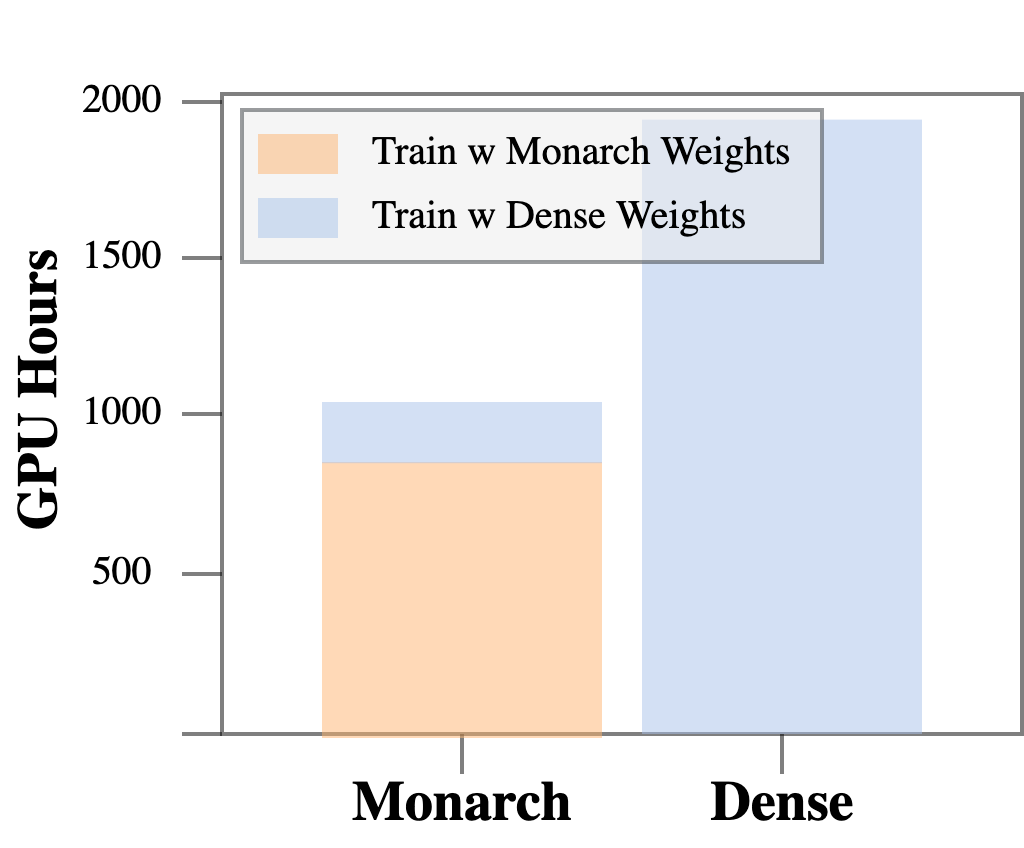
\includegraphics[width=.3\textwidth]{figures/rv_bar_temp.png}
  \vspace{-3mm}
  \caption{\label{fig:reverse_sparsification_bar}Time required (in A100 GPU hours) to reach the same perplexity (18.0)
    for GPT-2-small on OpenWebText.
    With ``reverse sparsification'', Monarch can speed up
    GPT-2 training by 2$\times$.\vspace{-1em}}
\end{figure}

We show that our Monarch approximation algorithm allows us to efficiently use
pretrained models, such as speeding up BERT finetuning on GLUE.

\paragraph{BERT finetuning.}
We take the BERT pretrained weights, approximate them with Monarch matrices,
and finetune the resulting model on the 9 GLUE tasks.
The results in \cref{table:bert_glue} shows that we obtain a Monarch finetuned
model with similar quality to the dense BERT model, but with 1.7$\times$ faster
finetuning speed.
This serves as a proof of concept, and we expect further speedup if additional model compression techniques are applied (e.g., quantization, kernel fusion).




\begin{table}[h]
  \small
  \centering
  \vspace{-5mm}
  \caption{\label{table:bert_glue}The performance of Monarch matrices in
    finetuning BERT on GLUE.}
  \setlength{\tabcolsep}{5pt}
  \vspace{1em}
  \iftoggle{arxiv}{}{
    \resizebox{\linewidth}{!}
  }
  {
  \begin{tabular}{@{}c||ccccccc@{}}
  \specialrule{.15em}{.05em}{.05em}
    Model&\multicolumn{1}{c}{GLUE (avg)}&\multicolumn{1}{c}{Speedup} &\multicolumn{1}{c}{Params} & \multicolumn{1}{c}{FLOPs} \\
    \specialrule{.15em}{.05em}{.05em}
    BERT-base & 78.6& - & 109M & 11.2G \\
    Monarch-BERT-base& 78.3& 1.5$\times$ & 55M & 6.2G  \\
    BERT-large & 80.4 & - & 335M & 39.5G \\
    Monarch-BERT-large & 79.6 & 1.7$\times$ & 144M & 14.6G  \\
    \specialrule{.15em}{.05em}{.05em}
  \end{tabular}
  }
  \vspace{-3mm}
\end{table}



	%!TEX root = ../main.tex

\section{Related Work}
\label{sec:related}

\textbf{State space models} have shown promise in modeling sequential data, including time series data~\citep{gu2022efficiently}, audio~\citep{goel2022s}, and visual data~\citep{nguyen2022s4nd}.
Our model builds off work on simplifying and parameterizing diagonal versions of S4~\citep{gu2022parameterization,gupta2022diagonal, gu2022train}.
Gated state spaces~\citep{mehta2022long} also aim to adapt SSMs to language modeling, but our results suggest that the GSS model does not perform as well as \hthree (or even as well as earlier SSMs like S4D).
The idea to combine SSMs with attention in hybrid models is not new; Mehta et al.~\citep{mehta2022long} also showed that interleaving attention with their GSS layer can improve performance, which we also validate on our OpenWebText experiments.
These positive results suggest that attention and SSMs are complementary, and that hybrid models may be a promising direction for future work.

\textbf{Large language foundation models}~\citep{bommasani2021opportunities} have demonstrated the power of scaling attention-based networks to billions of parameters and training them on trillions of tokens~\citep{hoffmann2022training}.
Understanding the mechanistic basis~\citep{elhage2021mathematical} behind these models may yield insights into better design choices for future models.
These and similar explorations have informed the design of \hthree and our selection of synthetic languages.
A number of recent works have also explored how to address the shortcomings of attention by approximating the attention computation~\citep{wang2020linformer,katharopoulos2020transformers, choromanski2020rethinking,tay2020long, kitaev2020reformer, daras2020smyrf}.
We believe these efforts are complementary to SSMs, and we are excited to see how they can be combined in future work.

\textbf{Linear attention}~\citep{katharopoulos2020transformers} and classical sequence models like RNNs serve as inspiration for \hthree.
Appendix~\ref{app:linear_attention} draws a direct connection between linear attention and LTI systems.
Luo et al.~\citep{luo2021stable} also propose a variant of linear attention that can achieve $O(n \log n)$ scaling in sequence length.
Appendix~\ref{sec:app_additional_experiments} evaluates linear attention on language modeling, and finds that it underperforms exact attention, whereas \hthree outperforms attention.
The multiplicative interactions in \hthree are reminiscent of gating mechanisms in LSTMs~\citep{hochreiter1996lstm} and GRUs~\citep{cho2014properties}, which suggests that architectural lessons from these sequence models may be useful for adapting SSMs to language modeling.
A number of algorithms for scaling attention to longer sequences have also been proposed, such as Transformer-XL~\citep{dai2019transformer}, Reformer~\citep{kitaev2020reformer}, Performer~\citep{choromanski2020rethinking}, and Perceiver AR~\citep{hawthorne2022general}.
Some of these approaches underperform exact attention on language modeling, and may be slower in wall-clock speed~\citep{dao2022flashattention}.
A thorough comparison of these alternatives to exact attention and how well they scale in model size and amount of training data is fruitful future work.

\textbf{FFT} algorithms are used in a wide variety of applications, including signal processing~\citep{oppenheim1978applications}, control theory~\citep{brogan1974modern}, and more.
Various algorithms for computing the FFT have existed for decades~\citep{oppenheim2001discrete}.
We hope our work on appealing to these classic algorithms to accelerate new applications such as learned SSMs will inspire future algorithmic exploration, even if hardware is not designed for them~\citep{hooker2021hardware}.

%%% Local Variables:
%%% mode: latex
%%% TeX-master: "../main"
%%% End:

    
Hyperbolic embeddings embed hierarchical information with high
fidelity and few dimensions. We explored the limits of this approach
by describing scalable, high quality algorithms. We hope the
techniques here encourage more follow-on work on the exciting
techniques of \citet{fb, ucl}. As future work, we hope to explore how
hyperbolic embeddings can be most effectively incorporated into downstream
tasks and applications.

    {\small
        \bibliography{mixup}
        \bibliographystyle{iclr2018}}
\end{document}
